% ============================================================================
% ACM e-Energy submission scaffold (acmart, two-column sigconf).
%
% This is the LaTeX harness that integrates the figures. The PROSE sections are
% placeholders (marked TODO) and are produced by the Research Engineer from
% acm_submission/paper_draft.md — replace each \section body, keep the figure
% includes. Compiles with the ACM acmart class.
%
% Figures live in paper/figures/ and are integrated via % ============================================================================
% ACM e-Energy — figures F7 / F8 for the results section.
% Include from the paper with:  % ============================================================================
% ACM e-Energy — figures F7 / F8 for the results section.
% Include from the paper with:  % ============================================================================
% ACM e-Energy — figures F7 / F8 for the results section.
% Include from the paper with:  \input{f7_f8_figures}
% Requires: \usepackage{graphicx}
%
% Generated by:
%   python -m experiments.paper_figures.make_paper_figures \
%       --runs <runs-root> --out experiments/figures
% <runs-root> layout: <root>/<regime>/<scenario>/<run_id>/result.json
% Figures are vector PDF (fonts embedded) with SVG + 600 dpi PNG previews.
% ACM convention: figure captions go BELOW the figure.
%
% Self-contained: the F7 PDF is committed at paper/figures/. Compile from the
% paper directory (\graphicspath resolves both locations), or drop the PDF next
% to your main .tex.
% ============================================================================

\graphicspath{{figures/}{../experiments/figures/}}

% ----------------------------------------------------------------------------
% F7 — cost vs. service by pricing regime  (full width, two-column layout)
% ----------------------------------------------------------------------------
\begin{figure*}[t]
  \centering
  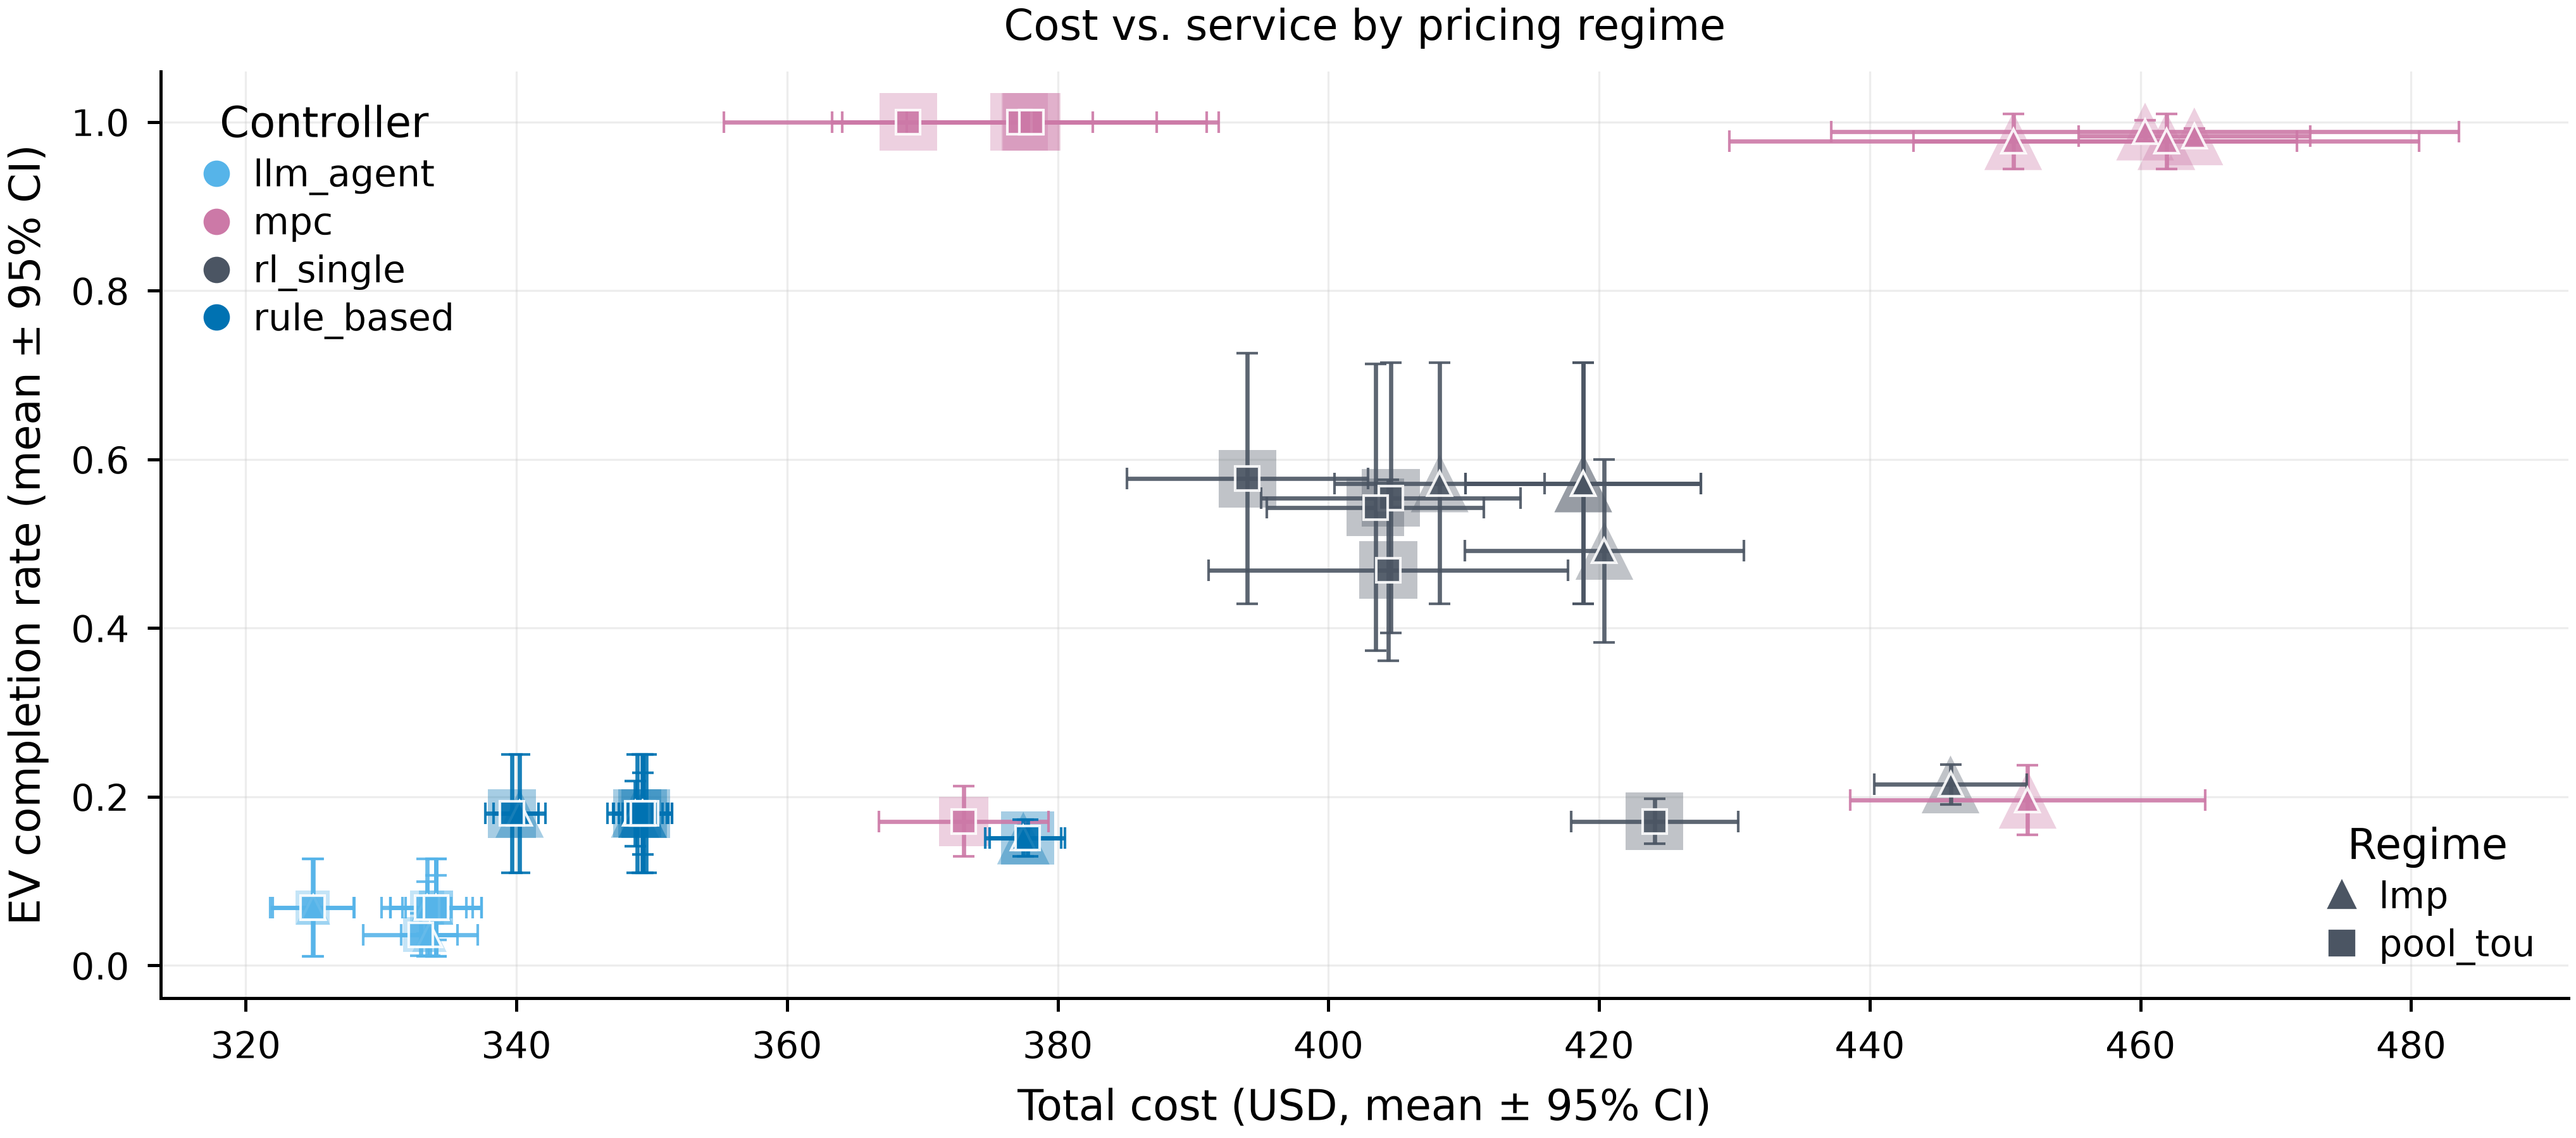
\includegraphics[width=\textwidth]{f7_cost_vs_service}
  \caption{Cost versus EV service across pricing regimes
    (\texttt{pool\_tou} vs.\ \texttt{lmp}): colour denotes the controller,
    marker shape the pricing regime, marker area the mean peak demand, and
    whiskers the 95\% confidence interval over seeds. Each point is one
    (regime, scenario, controller) cell ($N=310$ completed runs).}
  \label{fig:f7-cost-service}
\end{figure*}

% ----------------------------------------------------------------------------
% F8 — locational price dispersal over the week (single column)
%
% NOT EMITTED YET. F8 is gated on the LMP validity guard: a run may only feed
% the dispersal figure when cost_basis == lmp, the price mean is finite and
% positive, the measured spread is non-zero, and there are no OPF fallback
% steps. The current M1 \texttt{lmp} runs are fallback-dominated
% (power_flow_not_converged) with zero/negative measured spread, so drawing a
% "spread" figure now would misrepresent the physics. Uncomment once the guard
% passes and experiments/figures/f8_lmp_dispersal.pdf exists.
% ----------------------------------------------------------------------------
% \begin{figure}[t]
%   \centering
%   \includegraphics[width=\columnwidth]{f8_lmp_dispersal}
%   \caption{Locational marginal price dispersal over the week for the
%     congested scenario: community mean (line) with the min--max band across
%     buildings (shaded). The annotation reports the measured max spread and
%     states explicitly when prices are uniform.}
%   \label{fig:f8-lmp-dispersal}
% \end{figure}

% Requires: \usepackage{graphicx}
%
% Generated by:
%   python -m experiments.paper_figures.make_paper_figures \
%       --runs <runs-root> --out experiments/figures
% <runs-root> layout: <root>/<regime>/<scenario>/<run_id>/result.json
% Figures are vector PDF (fonts embedded) with SVG + 600 dpi PNG previews.
% ACM convention: figure captions go BELOW the figure.
%
% Self-contained: the F7 PDF is committed at paper/figures/. Compile from the
% paper directory (\graphicspath resolves both locations), or drop the PDF next
% to your main .tex.
% ============================================================================

\graphicspath{{figures/}{../experiments/figures/}}

% ----------------------------------------------------------------------------
% F7 — cost vs. service by pricing regime  (full width, two-column layout)
% ----------------------------------------------------------------------------
\begin{figure*}[t]
  \centering
  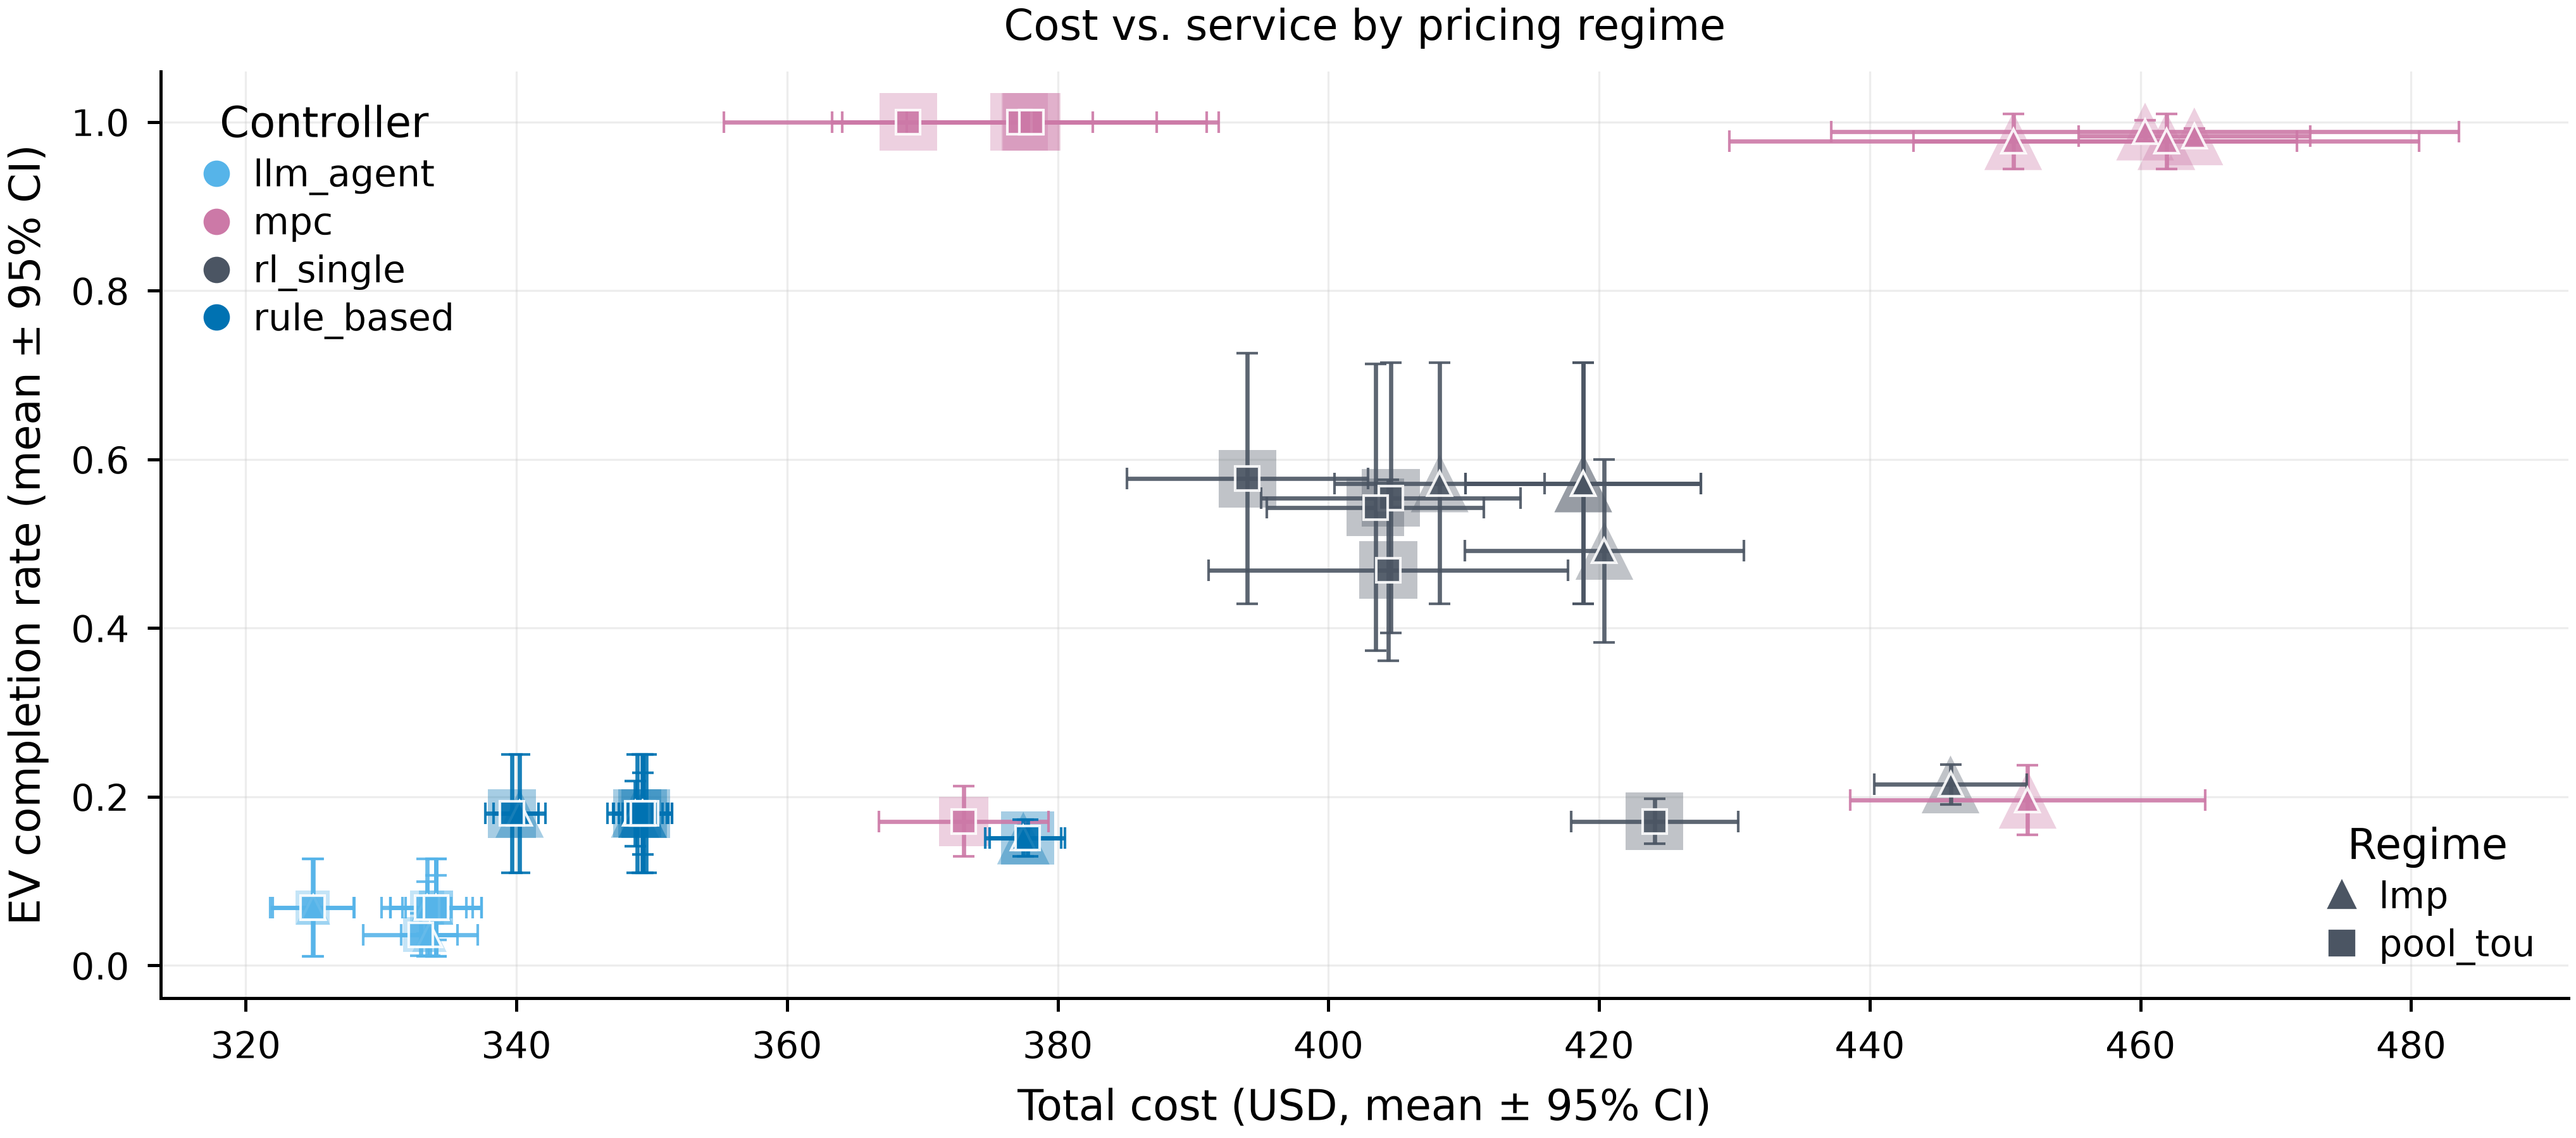
\includegraphics[width=\textwidth]{f7_cost_vs_service}
  \caption{Cost versus EV service across pricing regimes
    (\texttt{pool\_tou} vs.\ \texttt{lmp}): colour denotes the controller,
    marker shape the pricing regime, marker area the mean peak demand, and
    whiskers the 95\% confidence interval over seeds. Each point is one
    (regime, scenario, controller) cell ($N=310$ completed runs).}
  \label{fig:f7-cost-service}
\end{figure*}

% ----------------------------------------------------------------------------
% F8 — locational price dispersal over the week (single column)
%
% NOT EMITTED YET. F8 is gated on the LMP validity guard: a run may only feed
% the dispersal figure when cost_basis == lmp, the price mean is finite and
% positive, the measured spread is non-zero, and there are no OPF fallback
% steps. The current M1 \texttt{lmp} runs are fallback-dominated
% (power_flow_not_converged) with zero/negative measured spread, so drawing a
% "spread" figure now would misrepresent the physics. Uncomment once the guard
% passes and experiments/figures/f8_lmp_dispersal.pdf exists.
% ----------------------------------------------------------------------------
% \begin{figure}[t]
%   \centering
%   \includegraphics[width=\columnwidth]{f8_lmp_dispersal}
%   \caption{Locational marginal price dispersal over the week for the
%     congested scenario: community mean (line) with the min--max band across
%     buildings (shaded). The annotation reports the measured max spread and
%     states explicitly when prices are uniform.}
%   \label{fig:f8-lmp-dispersal}
% \end{figure}

% Requires: \usepackage{graphicx}
%
% Generated by:
%   python -m experiments.paper_figures.make_paper_figures \
%       --runs <runs-root> --out experiments/figures
% <runs-root> layout: <root>/<regime>/<scenario>/<run_id>/result.json
% Figures are vector PDF (fonts embedded) with SVG + 600 dpi PNG previews.
% ACM convention: figure captions go BELOW the figure.
%
% Self-contained: the F7 PDF is committed at paper/figures/. Compile from the
% paper directory (\graphicspath resolves both locations), or drop the PDF next
% to your main .tex.
% ============================================================================

\graphicspath{{figures/}{../experiments/figures/}}

% ----------------------------------------------------------------------------
% F7 — cost vs. service by pricing regime  (full width, two-column layout)
% ----------------------------------------------------------------------------
\begin{figure*}[t]
  \centering
  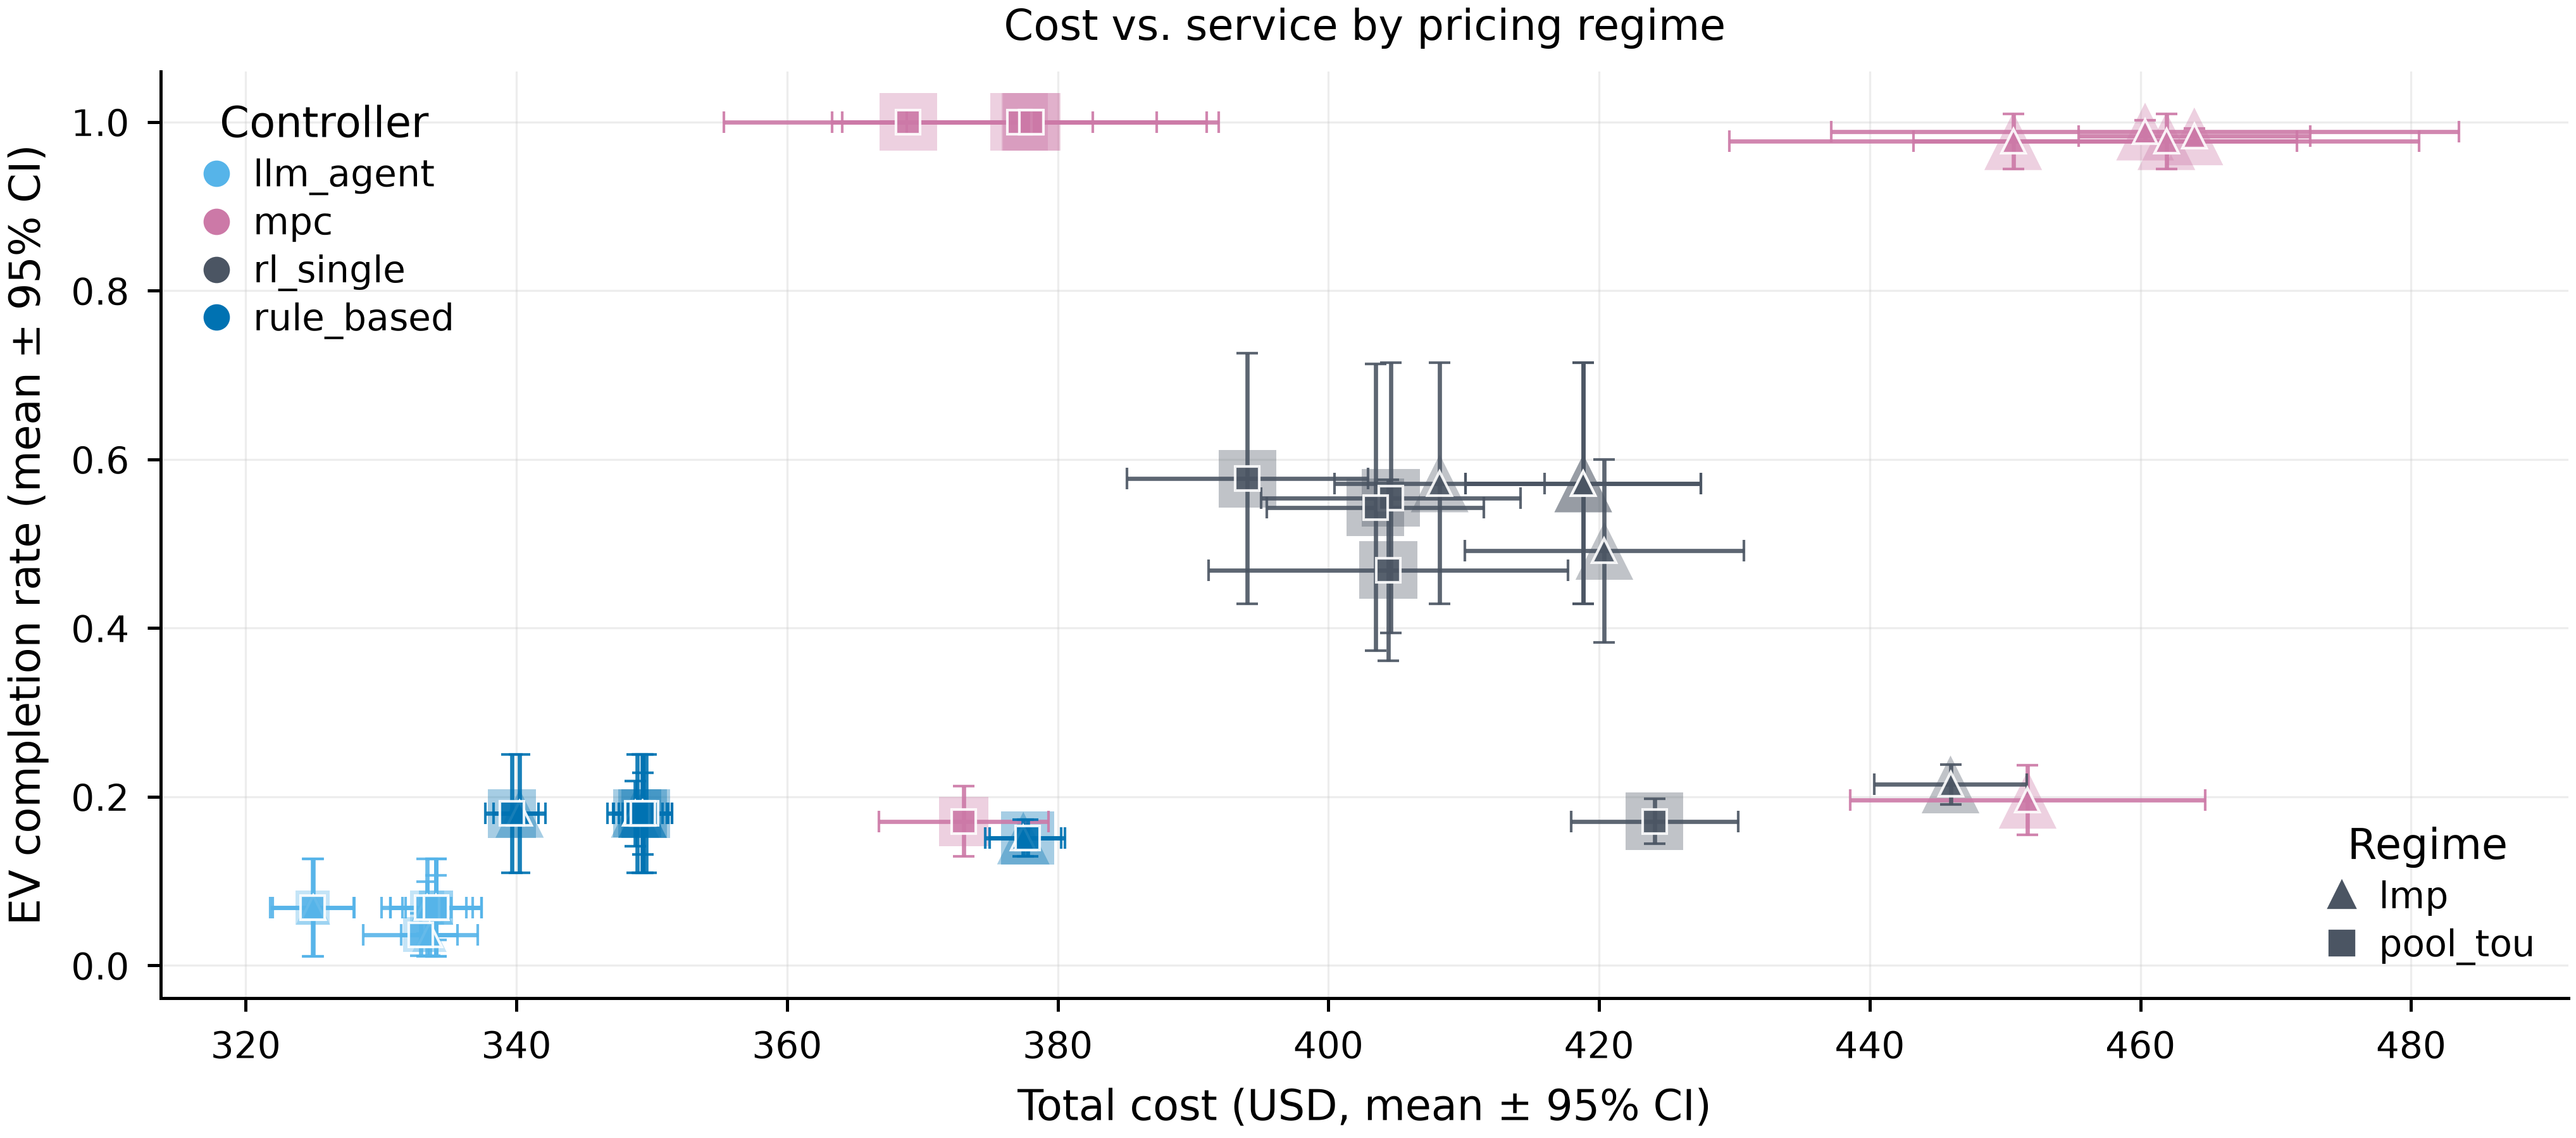
\includegraphics[width=\textwidth]{f7_cost_vs_service}
  \caption{Cost versus EV service across pricing regimes
    (\texttt{pool\_tou} vs.\ \texttt{lmp}): colour denotes the controller,
    marker shape the pricing regime, marker area the mean peak demand, and
    whiskers the 95\% confidence interval over seeds. Each point is one
    (regime, scenario, controller) cell ($N=310$ completed runs).}
  \label{fig:f7-cost-service}
\end{figure*}

% ----------------------------------------------------------------------------
% F8 — locational price dispersal over the week (single column)
%
% NOT EMITTED YET. F8 is gated on the LMP validity guard: a run may only feed
% the dispersal figure when cost_basis == lmp, the price mean is finite and
% positive, the measured spread is non-zero, and there are no OPF fallback
% steps. The current M1 \texttt{lmp} runs are fallback-dominated
% (power_flow_not_converged) with zero/negative measured spread, so drawing a
% "spread" figure now would misrepresent the physics. Uncomment once the guard
% passes and experiments/figures/f8_lmp_dispersal.pdf exists.
% ----------------------------------------------------------------------------
% \begin{figure}[t]
%   \centering
%   \includegraphics[width=\columnwidth]{f8_lmp_dispersal}
%   \caption{Locational marginal price dispersal over the week for the
%     congested scenario: community mean (line) with the min--max band across
%     buildings (shaded). The annotation reports the measured max spread and
%     states explicitly when prices are uniform.}
%   \label{fig:f8-lmp-dispersal}
% \end{figure}
.
% Challenge: ensure F8 stays commented until its LMP data-validity guard passes
% (see paper/README.md and docs/phase5_acm_figure_style.md).
% ============================================================================
\documentclass[sigconf]{acmart}

% --- Review options (uncomment one before submitting if required) -----------
% \documentclass[sigconf,review,anonymous]{acmart}   % double-anonymous review

\usepackage{booktabs}   % tables T1-T8
\usepackage{graphicx}
\usepackage{amsmath}

\begin{document}

\title{Service-Aware Energy Agents: Pricing Regimes, Failure Injection, and a
       Verified LLM Code-Agent Workflow for Community Energy Simulation}

% Author block — confirmed order (2026-11-02). Replace anonymous blocks if the
% venue runs double-anonymous review.
\author{Research Engineer}
\affiliation{\institution{Service-Aware-Energy-Agents Project / OpenBot Platform}}
\email{first.author@example.org}   % TODO real contact

\author{Backend/Simulation Engineer A}
\affiliation{\institution{Service-Aware-Energy-Agents Project / OpenBot Platform}}

\author{Backend/Simulation Engineer B}
\affiliation{\institution{Service-Aware-Energy-Agents Project / OpenBot Platform}}

\author{Frontend Engineer}
\affiliation{\institution{Service-Aware-Energy-Agents Project / OpenBot Platform}}

\author{Product Design Lead}
\affiliation{\institution{Service-Aware-Energy-Agents Project / OpenBot Platform}}

\author{QA/DevOps}
\affiliation{\institution{Service-Aware-Energy-Agents Project / OpenBot Platform}}

\author{Project Manager}
\affiliation{\institution{Service-Aware-Energy-Agents Project / OpenBot Platform}}
\email{corresponding@example.org}  % TODO real contact (corresponding author)

\renewcommand{\shortauthors}{Research Engineer et al.}

\begin{abstract}
% TODO (Research Engineer): abstract — not yet in the draft.
\end{abstract}

\maketitle

% ---------------------------------------------------------------------------
% Sections 1-4 (introduction / related work / system / method): TODO authors.
% Drop each as a \input{...} once available, e.g.
%   \input{sections/introduction}
% ---------------------------------------------------------------------------
\section{Introduction}
% TODO
\section{Related Work}
% TODO
\section{System and Method}
% TODO
\section{Experimental Setup}
% TODO — summary of scenarios (T1), controllers, seeds, pricing regimes.

% ---------------------------------------------------------------------------
% Section 5 — Results. Prose from acm_submission/paper_draft.md (§5.1-5.11).
% The figure include below is wired and ready; keep it here.
% ---------------------------------------------------------------------------
\section{Results}
% TODO (Research Engineer): §5.1-5.11 prose from paper_draft.md. Tables T1-T8
% via booktabs. The F7 figure is included by the line below; F8 stays gated.
% ============================================================================
% ACM e-Energy — figures F7 / F8 for the results section.
% Include from the paper with:  % ============================================================================
% ACM e-Energy — figures F7 / F8 for the results section.
% Include from the paper with:  % ============================================================================
% ACM e-Energy — figures F7 / F8 for the results section.
% Include from the paper with:  \input{f7_f8_figures}
% Requires: \usepackage{graphicx}
%
% Generated by:
%   python -m experiments.paper_figures.make_paper_figures \
%       --runs <runs-root> --out experiments/figures
% <runs-root> layout: <root>/<regime>/<scenario>/<run_id>/result.json
% Figures are vector PDF (fonts embedded) with SVG + 600 dpi PNG previews.
% ACM convention: figure captions go BELOW the figure.
%
% Self-contained: the F7 PDF is committed at paper/figures/. Compile from the
% paper directory (\graphicspath resolves both locations), or drop the PDF next
% to your main .tex.
% ============================================================================

\graphicspath{{figures/}{../experiments/figures/}}

% ----------------------------------------------------------------------------
% F7 — cost vs. service by pricing regime  (full width, two-column layout)
% ----------------------------------------------------------------------------
\begin{figure*}[t]
  \centering
  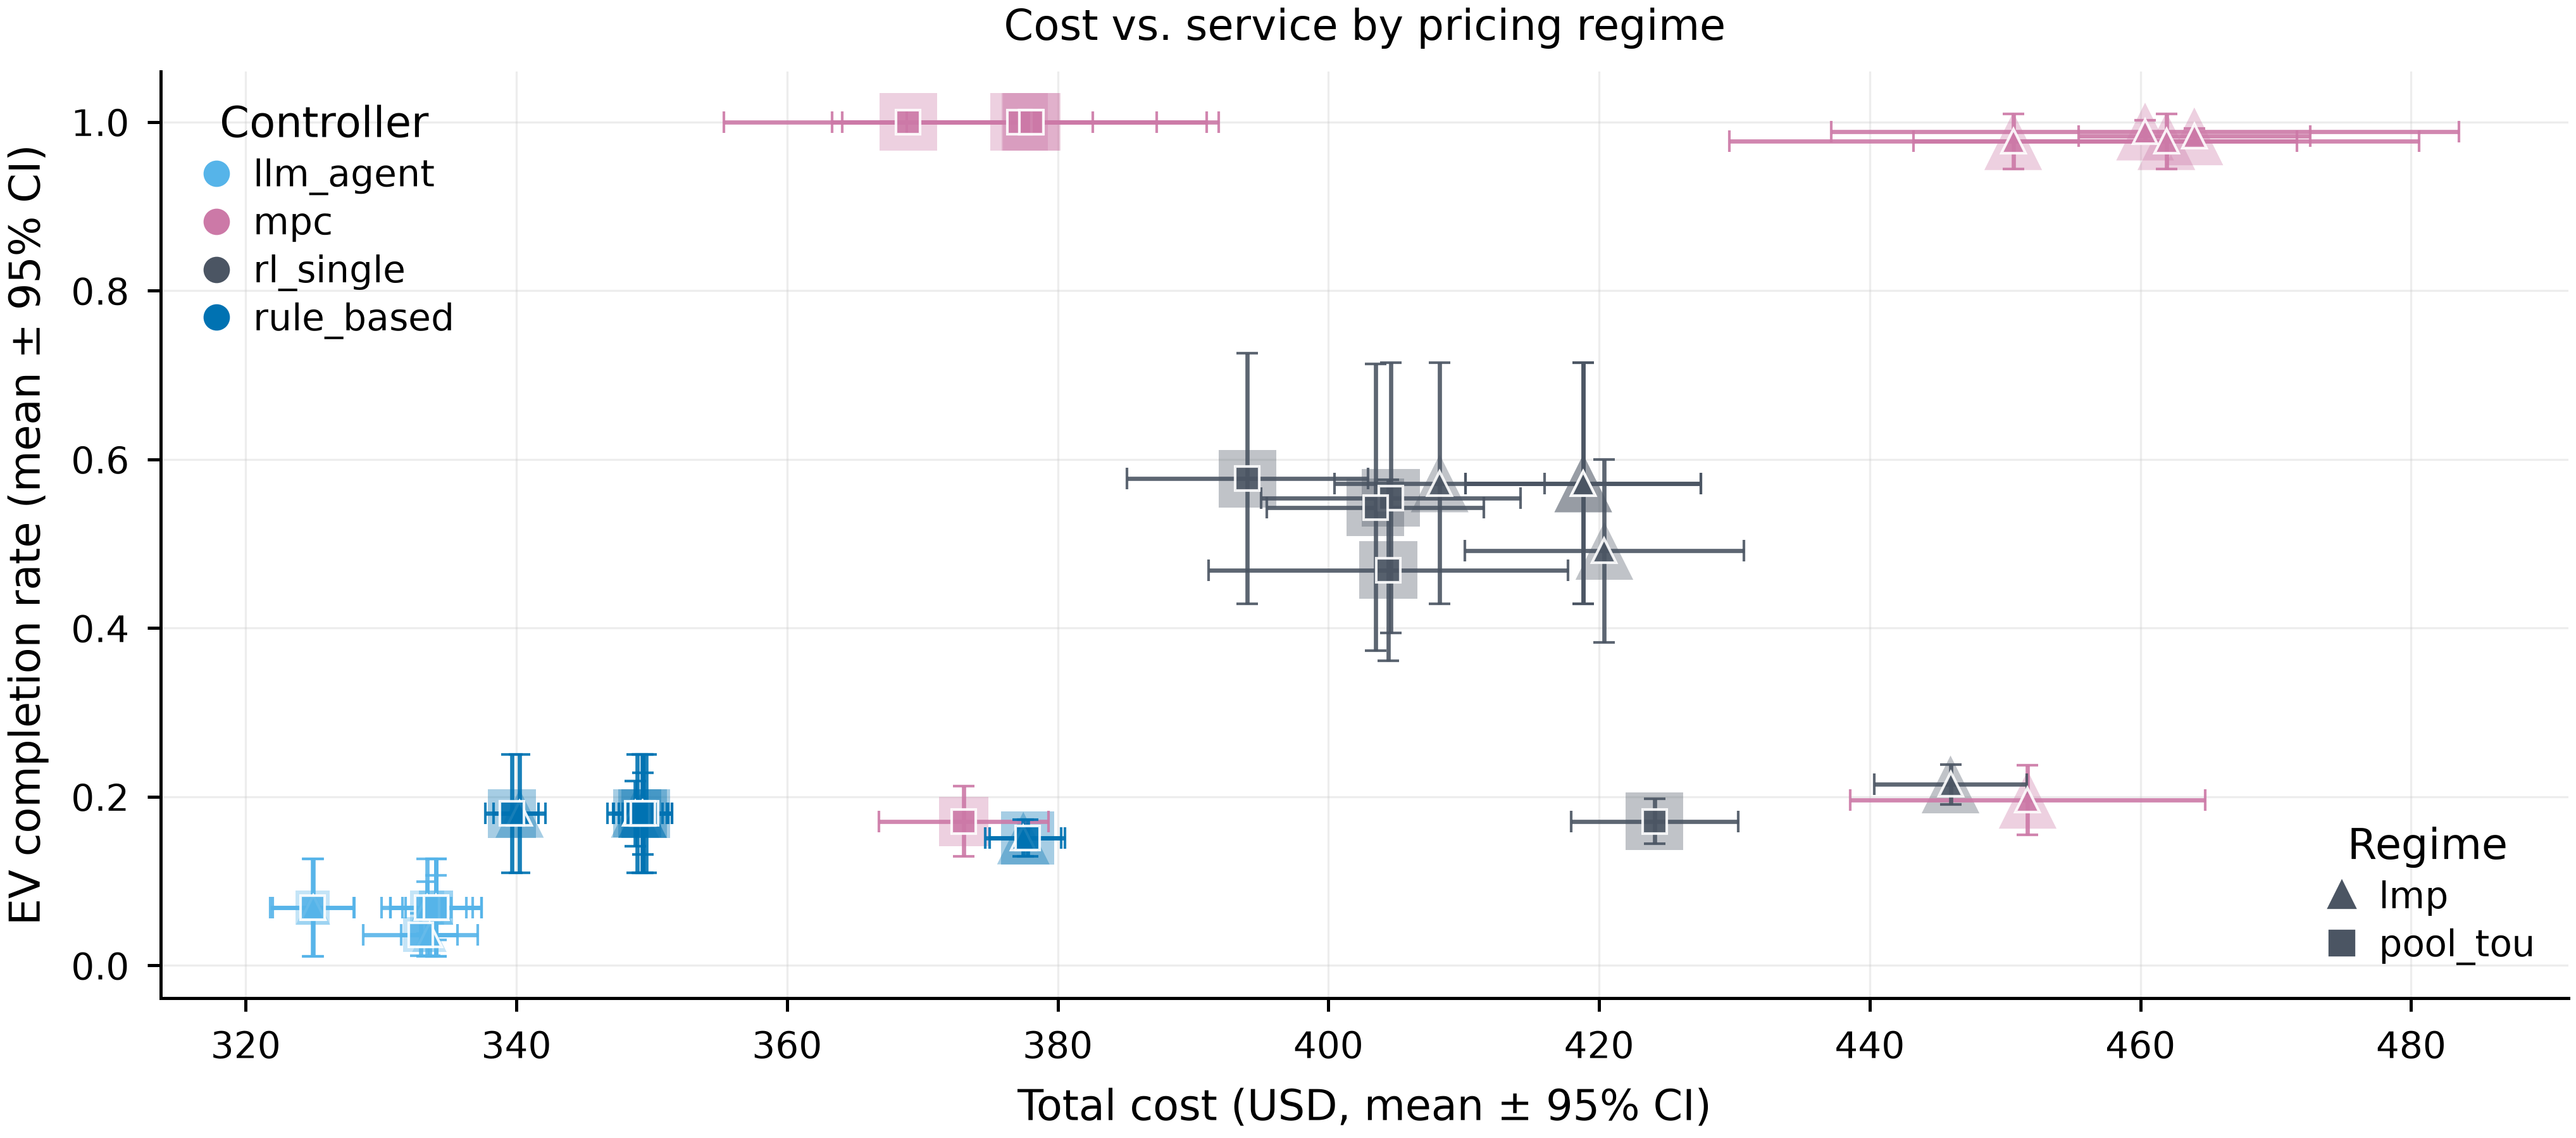
\includegraphics[width=\textwidth]{f7_cost_vs_service}
  \caption{Cost versus EV service across pricing regimes
    (\texttt{pool\_tou} vs.\ \texttt{lmp}): colour denotes the controller,
    marker shape the pricing regime, marker area the mean peak demand, and
    whiskers the 95\% confidence interval over seeds. Each point is one
    (regime, scenario, controller) cell ($N=310$ completed runs).}
  \label{fig:f7-cost-service}
\end{figure*}

% ----------------------------------------------------------------------------
% F8 — locational price dispersal over the week (single column)
%
% NOT EMITTED YET. F8 is gated on the LMP validity guard: a run may only feed
% the dispersal figure when cost_basis == lmp, the price mean is finite and
% positive, the measured spread is non-zero, and there are no OPF fallback
% steps. The current M1 \texttt{lmp} runs are fallback-dominated
% (power_flow_not_converged) with zero/negative measured spread, so drawing a
% "spread" figure now would misrepresent the physics. Uncomment once the guard
% passes and experiments/figures/f8_lmp_dispersal.pdf exists.
% ----------------------------------------------------------------------------
% \begin{figure}[t]
%   \centering
%   \includegraphics[width=\columnwidth]{f8_lmp_dispersal}
%   \caption{Locational marginal price dispersal over the week for the
%     congested scenario: community mean (line) with the min--max band across
%     buildings (shaded). The annotation reports the measured max spread and
%     states explicitly when prices are uniform.}
%   \label{fig:f8-lmp-dispersal}
% \end{figure}

% Requires: \usepackage{graphicx}
%
% Generated by:
%   python -m experiments.paper_figures.make_paper_figures \
%       --runs <runs-root> --out experiments/figures
% <runs-root> layout: <root>/<regime>/<scenario>/<run_id>/result.json
% Figures are vector PDF (fonts embedded) with SVG + 600 dpi PNG previews.
% ACM convention: figure captions go BELOW the figure.
%
% Self-contained: the F7 PDF is committed at paper/figures/. Compile from the
% paper directory (\graphicspath resolves both locations), or drop the PDF next
% to your main .tex.
% ============================================================================

\graphicspath{{figures/}{../experiments/figures/}}

% ----------------------------------------------------------------------------
% F7 — cost vs. service by pricing regime  (full width, two-column layout)
% ----------------------------------------------------------------------------
\begin{figure*}[t]
  \centering
  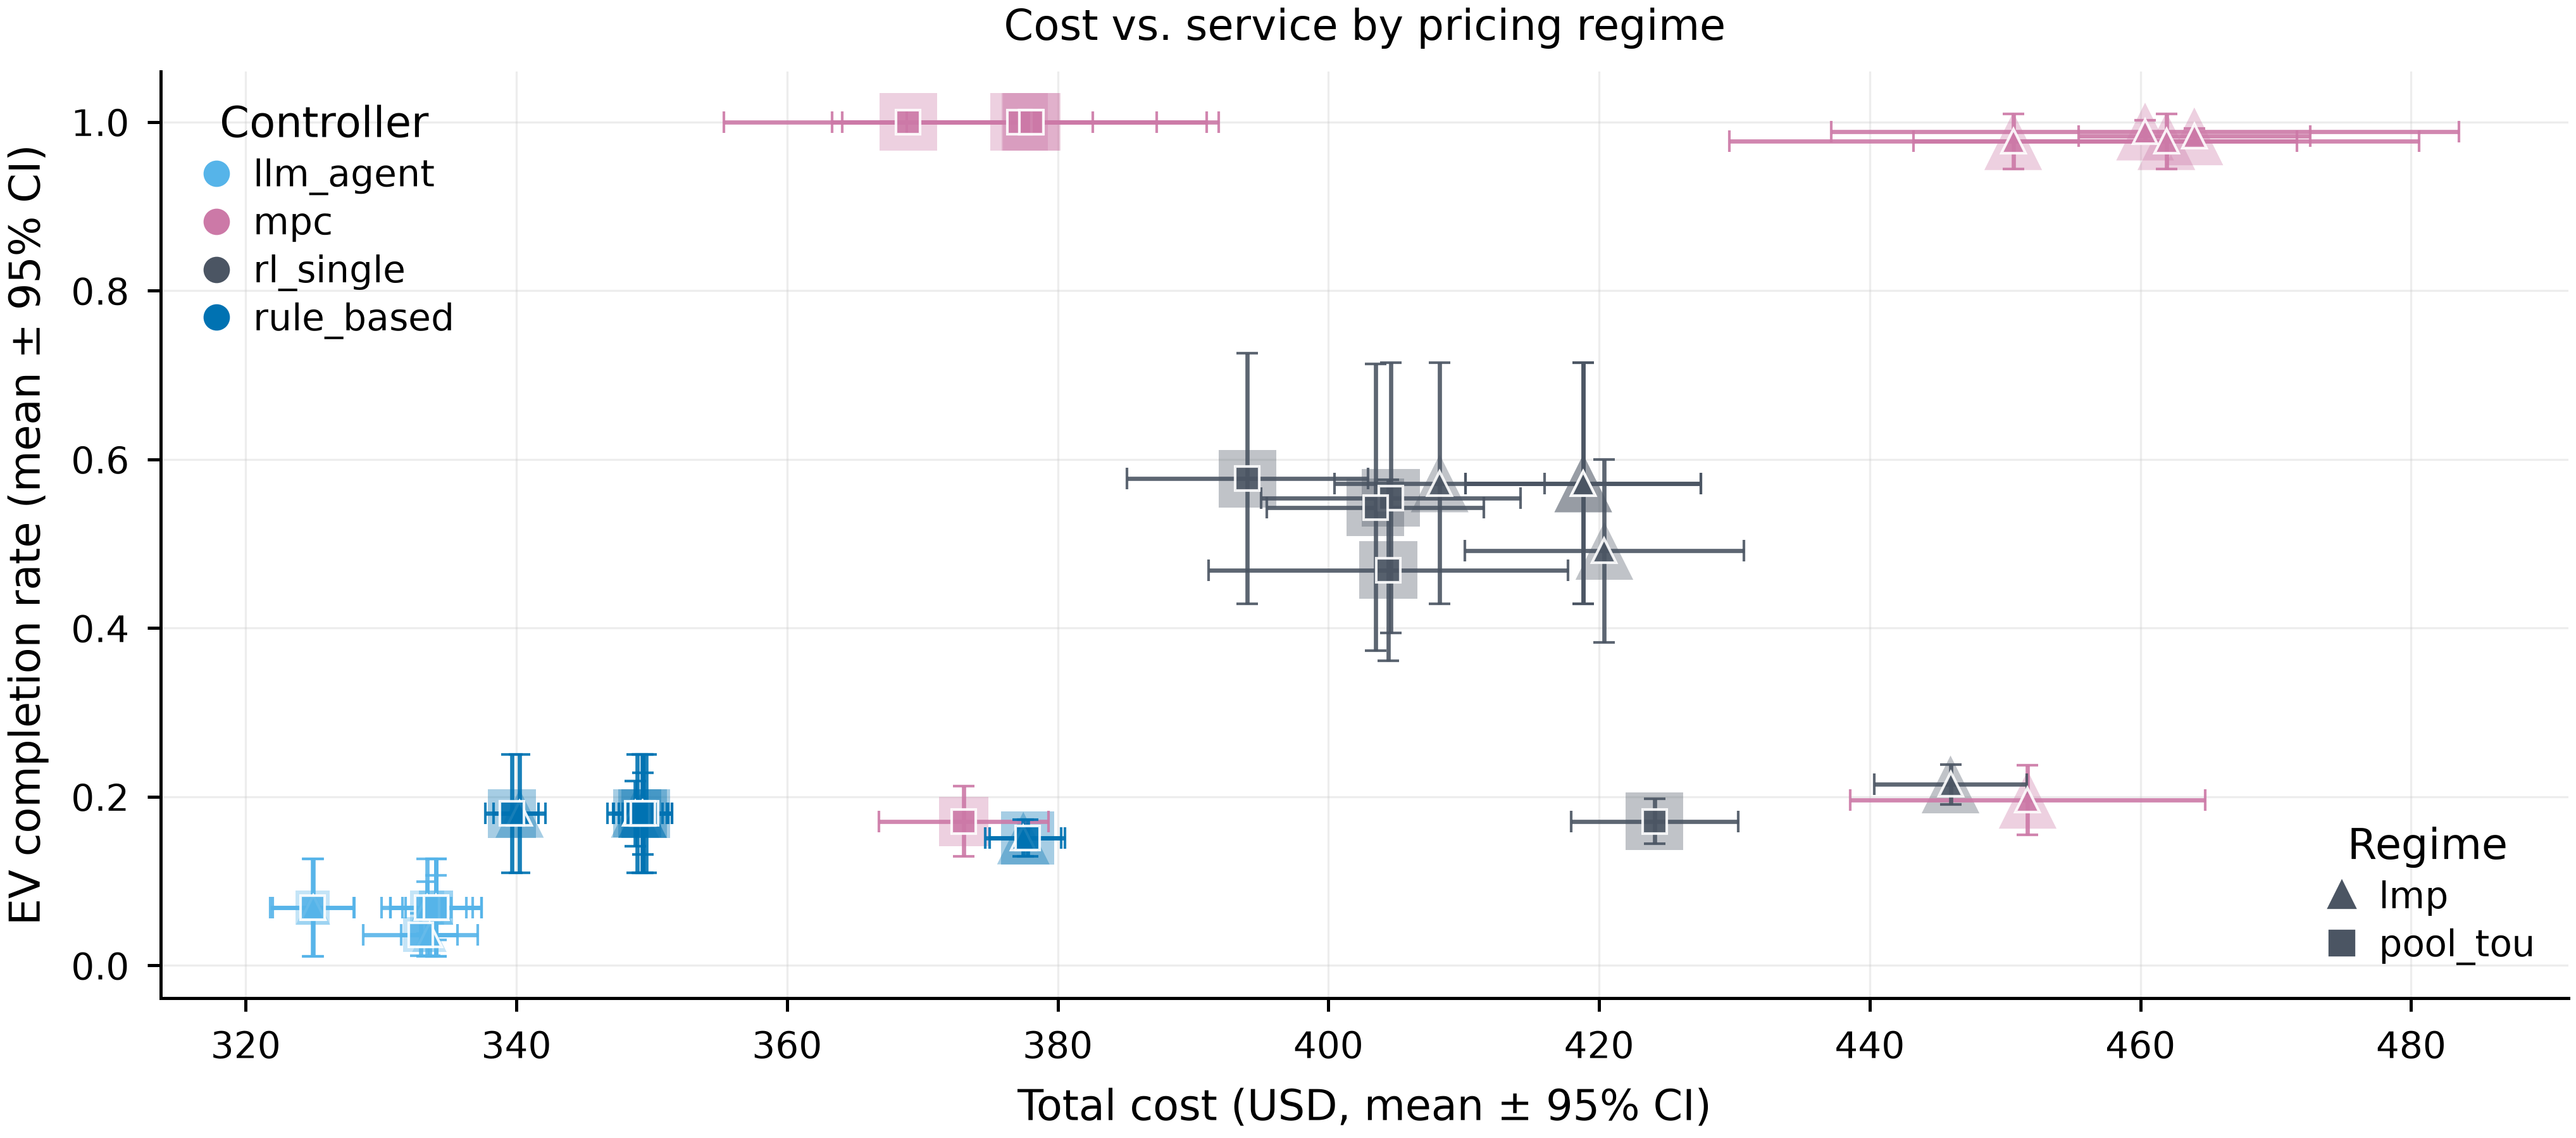
\includegraphics[width=\textwidth]{f7_cost_vs_service}
  \caption{Cost versus EV service across pricing regimes
    (\texttt{pool\_tou} vs.\ \texttt{lmp}): colour denotes the controller,
    marker shape the pricing regime, marker area the mean peak demand, and
    whiskers the 95\% confidence interval over seeds. Each point is one
    (regime, scenario, controller) cell ($N=310$ completed runs).}
  \label{fig:f7-cost-service}
\end{figure*}

% ----------------------------------------------------------------------------
% F8 — locational price dispersal over the week (single column)
%
% NOT EMITTED YET. F8 is gated on the LMP validity guard: a run may only feed
% the dispersal figure when cost_basis == lmp, the price mean is finite and
% positive, the measured spread is non-zero, and there are no OPF fallback
% steps. The current M1 \texttt{lmp} runs are fallback-dominated
% (power_flow_not_converged) with zero/negative measured spread, so drawing a
% "spread" figure now would misrepresent the physics. Uncomment once the guard
% passes and experiments/figures/f8_lmp_dispersal.pdf exists.
% ----------------------------------------------------------------------------
% \begin{figure}[t]
%   \centering
%   \includegraphics[width=\columnwidth]{f8_lmp_dispersal}
%   \caption{Locational marginal price dispersal over the week for the
%     congested scenario: community mean (line) with the min--max band across
%     buildings (shaded). The annotation reports the measured max spread and
%     states explicitly when prices are uniform.}
%   \label{fig:f8-lmp-dispersal}
% \end{figure}

% Requires: \usepackage{graphicx}
%
% Generated by:
%   python -m experiments.paper_figures.make_paper_figures \
%       --runs <runs-root> --out experiments/figures
% <runs-root> layout: <root>/<regime>/<scenario>/<run_id>/result.json
% Figures are vector PDF (fonts embedded) with SVG + 600 dpi PNG previews.
% ACM convention: figure captions go BELOW the figure.
%
% Self-contained: the F7 PDF is committed at paper/figures/. Compile from the
% paper directory (\graphicspath resolves both locations), or drop the PDF next
% to your main .tex.
% ============================================================================

\graphicspath{{figures/}{../experiments/figures/}}

% ----------------------------------------------------------------------------
% F7 — cost vs. service by pricing regime  (full width, two-column layout)
% ----------------------------------------------------------------------------
\begin{figure*}[t]
  \centering
  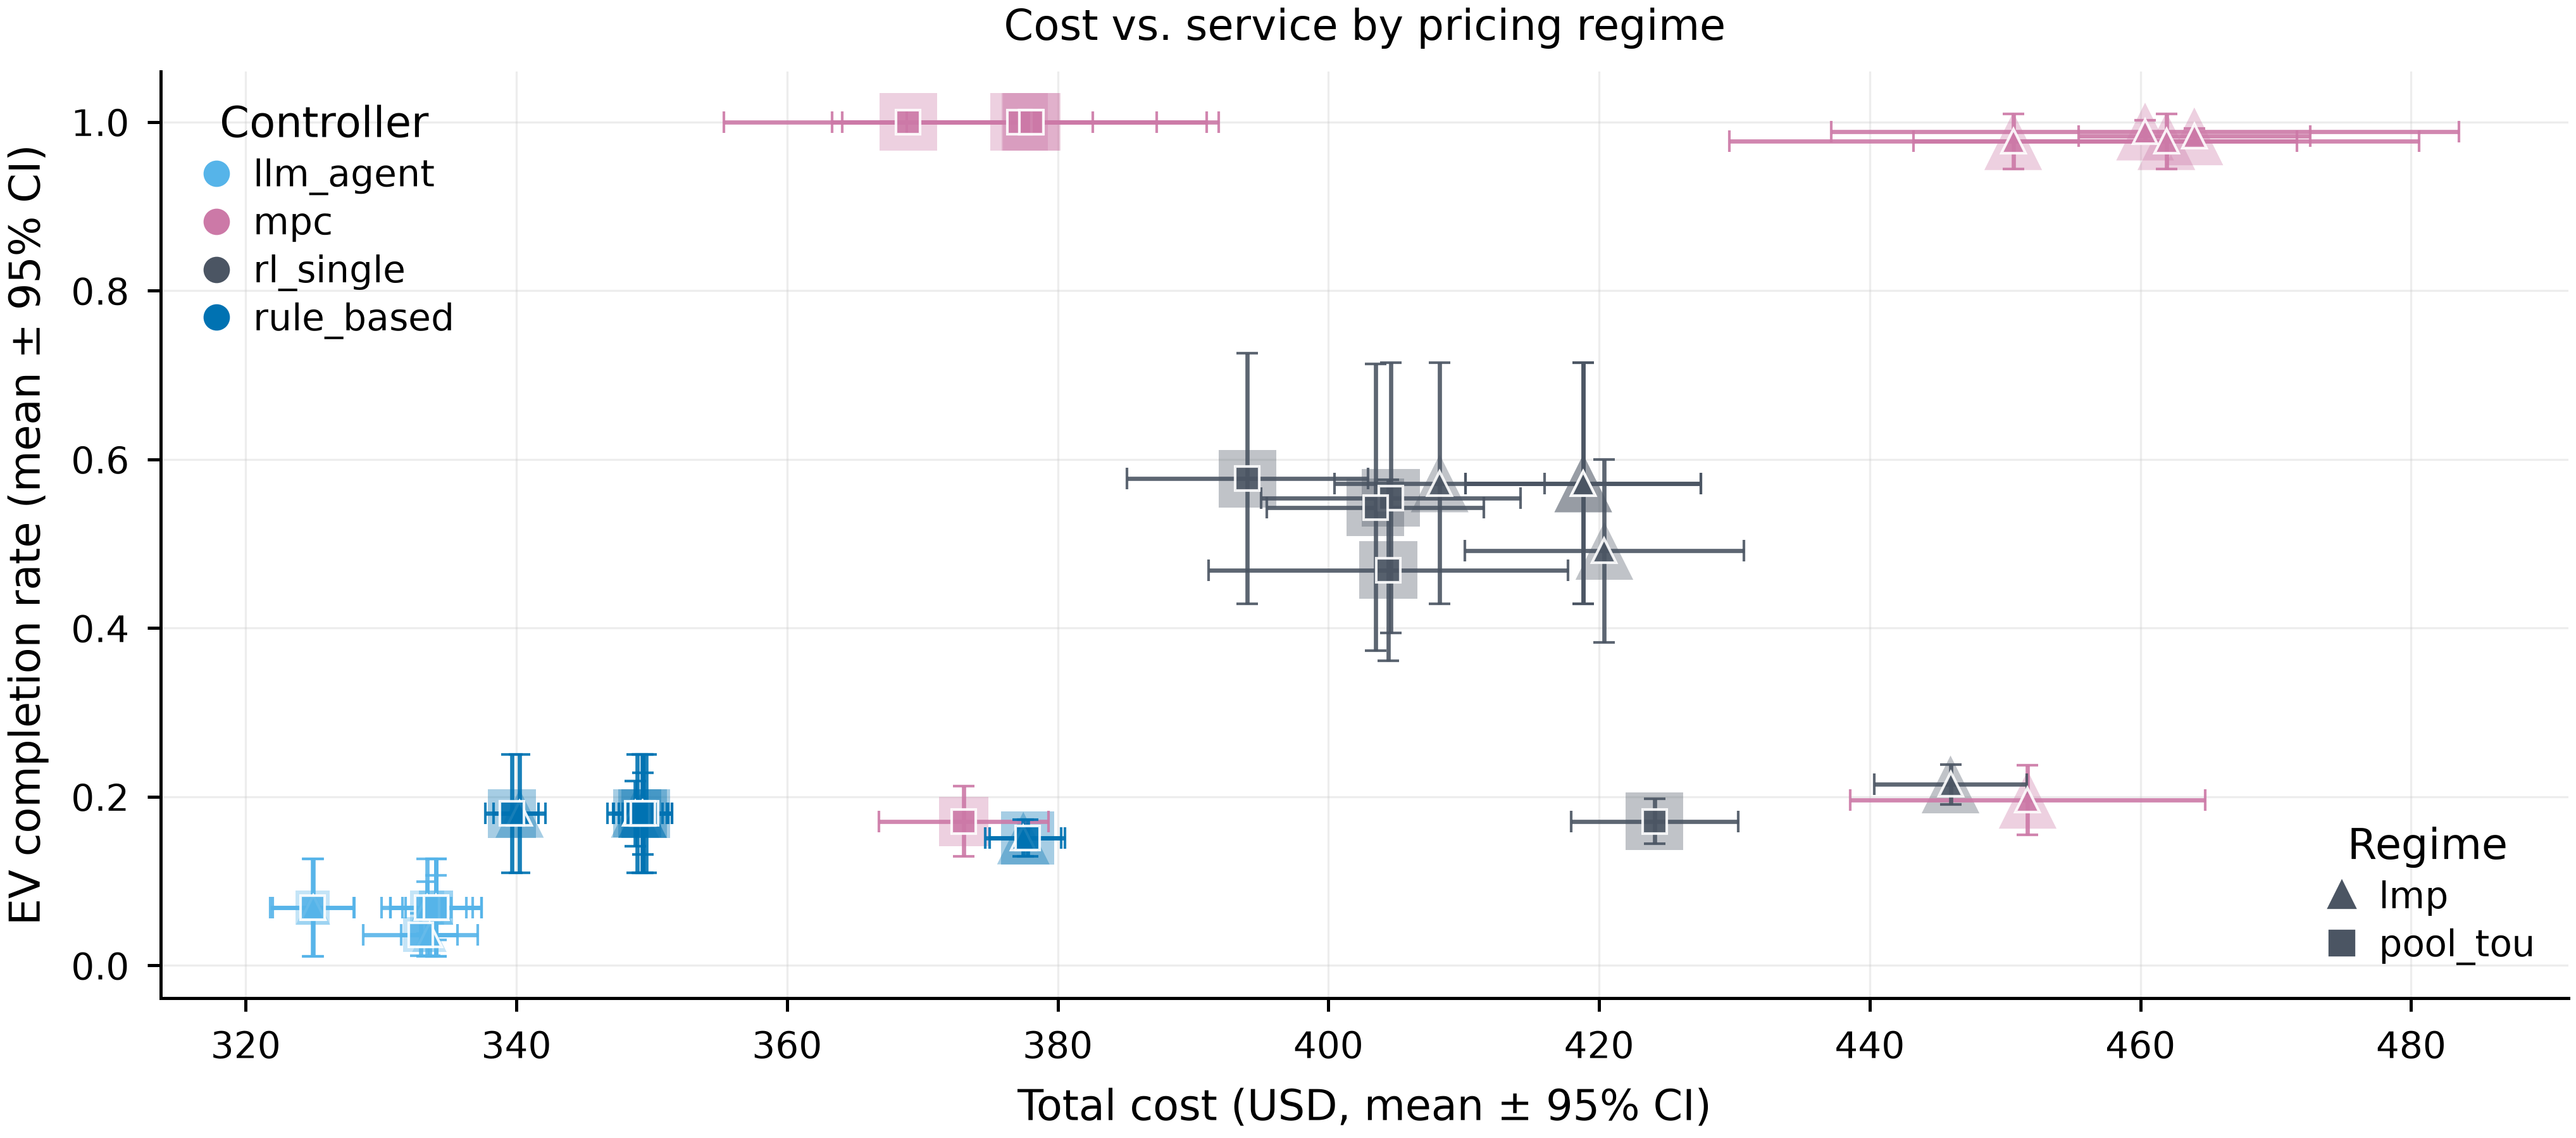
\includegraphics[width=\textwidth]{f7_cost_vs_service}
  \caption{Cost versus EV service across pricing regimes
    (\texttt{pool\_tou} vs.\ \texttt{lmp}): colour denotes the controller,
    marker shape the pricing regime, marker area the mean peak demand, and
    whiskers the 95\% confidence interval over seeds. Each point is one
    (regime, scenario, controller) cell ($N=310$ completed runs).}
  \label{fig:f7-cost-service}
\end{figure*}

% ----------------------------------------------------------------------------
% F8 — locational price dispersal over the week (single column)
%
% NOT EMITTED YET. F8 is gated on the LMP validity guard: a run may only feed
% the dispersal figure when cost_basis == lmp, the price mean is finite and
% positive, the measured spread is non-zero, and there are no OPF fallback
% steps. The current M1 \texttt{lmp} runs are fallback-dominated
% (power_flow_not_converged) with zero/negative measured spread, so drawing a
% "spread" figure now would misrepresent the physics. Uncomment once the guard
% passes and experiments/figures/f8_lmp_dispersal.pdf exists.
% ----------------------------------------------------------------------------
% \begin{figure}[t]
%   \centering
%   \includegraphics[width=\columnwidth]{f8_lmp_dispersal}
%   \caption{Locational marginal price dispersal over the week for the
%     congested scenario: community mean (line) with the min--max band across
%     buildings (shaded). The annotation reports the measured max spread and
%     states explicitly when prices are uniform.}
%   \label{fig:f8-lmp-dispersal}
% \end{figure}


\section{Discussion and Limitations}
% TODO (Research Engineer): §5.9 null ablation discussion, §5.11 threat model,
% and the ordered caveats list.

\section{Conclusion}
% TODO

\begin{acks}
% TODO optional
\end{acks}

\bibliographystyle{ACM-Reference-Format}
\bibliography{references}   % TODO: references.bib from the authors

\end{document}
